\documentclass[smaller]{beamer}
\usetheme[english]{Berlin}
%\usepackage{ngerman}
\usepackage[ngerman]{babel}
\useoutertheme{infolines}
\beamertemplatenavigationsymbolsempty
\setbeamertemplate{caption}[numbered]
\usepackage{pgfplots,tikz,subfigure}
\usepackage{amsmath,amsthm}
\usepackage{hyperref,graphics,graphicx,color,algorithm,algorithmic,enumerate}
\usepackage{mymacros,wrapfig,relsize}
\usepackage{pict2e}
\usepackage[utf8x]{inputenc}
\usepackage{csquotes}

\newcommand{\ri}{\mathrm{i}}
\newcommand{\T}{\mathsf{T}}
\renewcommand{\H}{\mathsf{H}}
\newcommand{\eps}{\varepsilon}
\newcommand{\To}{\rightarrow}
\newcommand{\sddots}{\scalebox{0.6}{$\ddots$}}
\usepackage[pdf]{pstricks}
\usepackage{sansmathfonts}
\usepackage{eurosym}
\usepackage{ulem}
\renewcommand{\O}{\mathcal{O}}
\DeclareMathOperator{\opt}{OPT}
\DeclareMathOperator{\copt}{Compute-OPT}
\DeclareMathOperator{\icopt}{Iterative-Compute-OPT}
\DeclareMathOperator{\ssum}{Subset-Sum}
%\usepackage{arev}
%\renewcommand\familydefault{\sfdefault}

\DeclareMathOperator{\loc}{loc}
\DeclareMathOperator{\rank}{rank}
\DeclareMathOperator{\RE}{Re}
\DeclareMathOperator{\IM}{Im}
\DeclareMathOperator{\In}{In}
\DeclareMathOperator{\im}{im}
\DeclareMathOperator{\Gl}{Gl}
\DeclareMathOperator{\spa}{span}
\DeclareMathOperator{\ext}{{ext}}
\DeclareMathOperator{\ind}{ind}
\DeclareMathOperator{\normalrank}{normalrank}
\DeclareMathOperator{\essup}{ess\,sup}
\DeclareMathOperator{\vect}{vec}

\newcommand{\re}{\mathrm{e}}
\newcommand{\ddt}{\tfrac{\mathrm{d}}{\mathrm{d}t}}
\newcommand{\sys}[4]{\left[\begin{array}{c|c} #1 & #2 \\ \hline #3 & #4 \end{array}\right]}

\renewcommand{\tilde}{\widetilde}
\renewcommand{\hat}{\widehat}


\title[]{Optimierung f\"ur Studierende der Informatik}
\subtitle{-- 12. Vorlesung --}
\author[Matthias Voigt]{\textbf{Matthias Voigt$^{1,2}$}}
\institute[]{
\begin{columns}
%\begin{center}
\column{0.45\textwidth}{\centering {$^1$Universit\"at Hamburg \\ Fachbereich Mathematik \\ Hamburg \\ }}
\column{0.45\textwidth}{\centering {$^2$Technische Universit\"at Berlin \\ Institut f\"ur Mathematik \\ Berlin  \\}}
%\end{center}
\end{columns}
}
\date[]{Universit\"at Hamburg
\begin{columns}
\column{0.45\textwidth}{\centering \includegraphics[width = 1.2\textwidth]{uhh-logo.png}\\}
\end{columns}
}

\definecolor{tucgreen}{rgb}{0.0,0.5,0.27}
\definecolor{tucred}{rgb}{0.75,0,0}
\definecolor{tucorange}{rgb}{1.0,.5625,0}
\definecolor{mpired}{HTML}{990000}
\definecolor{mpigreen}{HTML}{5C871D}
\definecolor{mpiblue}{HTML}{006AA9}
\definecolor{mpibg1}{HTML}{5D8B8A}
\definecolor{mpibg2}{HTML}{BFDFDE}
\definecolor{mpibg3}{HTML}{A7C1C0}
\definecolor{mpibg4}{HTML}{7DA9A8}
\definecolor{mpigrey}{rgb}{0.9294,0.9294,0.8784}

\newcommand{\Z}{\mathbb{Z}}

\begin{document}

\maketitle

\begin{frame}
\frametitle{Einige Bezeichnungen (Wiederholung)}
Wir beginnen mit der \alert{Zusammenstellung einiger Bezeichnungen}. \\ \vspace*{0.2cm}

Ist ein Graph $G$ gegeben, so bezeichnen wir die Knotenmenge von $G$ mit $V(G)$; $E(G)$ bezeichnet die Kantenmenge von $G$. Für $X \subseteq V(G)$ sei mit $\delta(X)$ die Menge derjenigen Kanten $e \in E(G)$ bezeichnet, für die gilt: Genau ein Endpunkt von $e$ liegt in $X$ (siehe Zeichnung).

\begin{center}
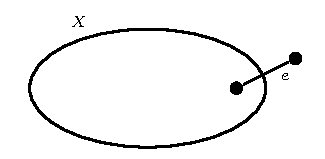
\includegraphics{fig82.pdf}
\end{center}

Soll betont werden, dass wir uns auf den Graphen $G$ beziehen, so schreiben wir $\delta_G(X)$ anstelle von $\delta(X)$.

\end{frame}

\begin{frame}
\frametitle{Ein Hilfssatz}
 \textbf{Hilfssatz:} Es sei $(G,c)$ eine Instanz des Minimum-Spanning-Tree-Problems und $T$ sei ein aufspannender Baum von $G$. \alert{Dann sind die folgenden vier Aussagen äquivalent:}
	\begin{enumerate}[a)]
		\item $T$ ist optimal.
		
		\item Für jede Kante $e = \big\{ x,y \big\} \in E(G) \setminus E(T)$ gilt: Keine Kante des $x,y$-Pfades in $T$ hat höheres Gewicht als $e$.
		
		\item Für jedes $e \in E(T)$ gilt: Ist $B$ eine der beiden Zusammenhangskomponenten von $T-e$, so ist $e$ eine Kante aus $\delta(V(B))$, die unter allen Kanten aus $\delta(V(B))$ minimales Gewicht hat.
		
		\item Es existiert eine Reihenfolge $e_1,\ldots,e_{n-1}$ der Kanten von $T$ mit der Eigenschaft, dass es zu jeder der Kanten $e_i$ eine Menge $X \subseteq V(G)$ gibt, die Folgendes erfüllt:
		\begin{itemize}
			\item $e_i \in \delta(X)$ und unter allen Kanten aus $\delta(X)$ hat $e_i$ minimales Gewicht;
			
			\item $e_j \notin \delta(X)$ für alle $j \in \big\{ 1,\ldots, i-1\big\}$. 
		\end{itemize}
	\end{enumerate}
\end{frame}

\begin{frame}
\frametitle{Veranschaulichung der Bedingung b)}
 Der $x,y$-Pfad in $T$ besteht aus den Kanten $e_1,e_2,e_3$. Ist b) erfüllt, so gilt $c(e_i) \leq c(e)$ für alle drei Kanten $e_i$.

%\begin{figure}[H]
\begin{center}
%	\centering
\includegraphics[scale=0.85]{fig83.pdf}
\end{center}
%\end{figure}
\end{frame}

\begin{frame}
\frametitle{Veranschaulichung der Bedingung c)}
Ist c) erfüllt, so gilt $c(e) \leq c(f)$ für alle Kanten $f \in \delta(V(B))$.

\begin{center}
 \includegraphics[scale = 0.85]{fig84.pdf}
\end{center}

\end{frame}

\begin{frame}
\frametitle{Veranschaulichung der Bedingung d)}
 Es wird angenommen, dass eine Reihenfolge $e_1,\ldots,e_{n-1}$ wie in d) gegeben ist; $e_1,e_2,e_3,e_4$ seien die ersten vier Kanten dieser Reihenfolge und es gelte $i=4$. Die Menge $X \subseteq V(G)$ sei die zu $e_4$ gehörige Menge. \\ \vspace*{0.2cm}
 
 Es gilt $e_4 \in \delta(X)$, aber $e_1,e_2,e_3 \notin \delta(X)$. Außerdem hat $e_4$ minimales Gewicht unter allen Kanten aus $\delta(X)$.
 
\begin{center}
 \includegraphics{fig85.pdf}
\end{center}
\end{frame}

\begin{frame}
\frametitle{Beweis des Hilfssatzes}
\textbf{Beweis des Hilfssatzes:} Wir weisen die Äquivalenz der vier Aussagen dadurch nach, dass wir nacheinander die folgenden Implikationen zeigen:
 \begin{equation*}
 \text{a)} \Rightarrow \text{b)} \Rightarrow \text{c)} \Rightarrow \text{d)} \Rightarrow \text{a)}.
 \end{equation*}
 \medskip
\structure{\textbf{a) $\Rightarrow$ b):}} Wir setzen voraus, dass $T$ optimal ist, und haben zu zeigen, dass $T$ die Pfadbedingung b) erfüllt. Hierzu nehmen wir an, dass \alert{b) nicht gilt und führen diese Annahme zum Widerspruch.} \medskip

Aufgrund der Annahme, dass b) nicht gilt, gibt es eine Kante $e=\{x,y\} \in E(G) \setminus E(T)$ und eine Kante $e'$ auf dem $x,y$-Pfad von $T$ mit $c(e') > c(e)$. Dann ist aber $(T-e')+e$ ein aufspannender Baum von $G$ mit kleineren Kosten als $T$ -- im Widerspruch zur Voraussetzung, dass $T$ optimal ist.

\end{frame}

\begin{frame}
\frametitle{Beweis des Hilfssatzes}
\structure{\textbf{b) $\Rightarrow$ c):}} Wir setzen voraus, dass $T$ die Pfadbedingung b) erfüllt, und haben zu zeigen, dass dann für $T$ auch die Schnittbedingung c) erfüllt ist. Wir gehen analog zum Beweis der Implikation a) $\Rightarrow$ b) vor: \alert{Es wird angenommen, dass c) nicht gilt, und nachgewiesen, dass sich aus dieser Annahme ein Widerspruch ergibt.} \medskip

Aufgrund der Annahme, dass c) nicht gilt, gibt es eine Kante $e \in E(T)$, eine Komponente\footnote{Es ist üblich, statt \structure{Zusammenhangskomponente} nur \structure{Komponente}\index{Komponente} zu sagen.} $B$ von $T-e$ sowie eine Kante $f=\bigl\{ x,y\bigr\} \in \delta(V(B))$, so dass $c(f) < c(e)$ gilt.\medskip

Man beachte, dass der $x,y$-Pfad $P$ in $T$ eine Kante aus $\delta_G(V(B))$ enthalten muss. Die einzige Kante von $G$, die sowohl in $T$ als auch in $\delta_G(V(B))$ liegt, ist jedoch $e$. Die Kante $e$ liegt also auf $P$. \medskip

Aus b) folgt demnach $c(e) \leq c(f)$ -- im Widerspruch zu $c(f) < c(e)$.

\medskip

\end{frame}

\begin{frame}
\frametitle{Beweis des Hilfssatzes}
\structure{\textbf{c) $\Rightarrow$ d):}} Wir setzen voraus, dass c) gilt und wählen eine \alert{beliebige} Reihenfolge $e_1,\ldots,e_{n-1}$ der Kanten von $T$. Wir betrachten die Kante $e_i$ ($i$-te Kante in dieser Reihenfolge) und wählen eine der beiden Komponenten $B$ von $T-e_i$.

 Wir setzen $X = V(B)$. Aufgrund von c) gilt dann 
 \begin{enumerate}[i)]
   \item $e_i \in \delta(X)$ und unter allen Kanten aus $\delta(X)$ hat $e_i$ minimales Gewicht. Außerdem gilt $e_j \not\in \delta(X)$ für alle $j \neq i$. Somit ist auch die zweite Bedingung  von d) erfüllt:
  \item $e_j \notin \delta(X)$ für alle $j \in \{1, \ldots, i-1\}$.
 \end{enumerate}
Damit ist dann c) $\Rightarrow$ d) nachgewiesen.
\end{frame}

\begin{frame}
\frametitle{Beweis des Hilfssatzes}
\structure{\textbf{d) $\Rightarrow$ a):}} Es sei $e_1,\ldots,e_{n-1}$ eine Reihenfolge der Kanten von $T$, für die d) erfüllt ist. Wir haben nachzuweisen, dass $T$ optimal ist. Hierzu betrachten wir einen optimalen Baum $T^*$. \medskip

Der Baum $T^*$ sei unter allen optimalen Bäumen so gewählt, dass $T^*$ ein \alert{möglichst langes Anfangsstück} der Folge $e_1,\ldots,e_{n-1}$ enthält.\medskip

Falls $T^*$ sämtliche Kanten $e_1,\ldots,e_{n-1}$ enthält, so folgt $T=T^*$, da $T^*$ (wegen $|E(T^*)| = n-1$) keine weiteren Kanten enthalten kann. \alert{In diesem Fall sind wir fertig.} \medskip

\alert{Andernfalls} bezeichnen wir mit $h$ den kleinsten Index aus $\bigl\{ 1,\ldots,n-1 \bigr\}$, für den $e_h \notin E(T^*)$ gilt.

\end{frame}

\begin{frame}
 \frametitle{Beweis des Hilfssatzes}
 \alert{Hieraus leiten wir nun einen Widerspruch ab. (Man beachte: Gelingt uns dies, so sind wir fertig.)} \medskip

Da d) für die Reihenfolge $e_1,\ldots,e_{n-1}$ erfüllt ist, gibt es ein $X \subseteq V(G)$, für das Folgendes erfüllt ist:
\begin{itemize}
	\item $e_h \in \delta(X)$ und unter allen Kanten aus $\delta(X)$ hat $e_h$ minimales Gewicht;
	\item $e_j \notin \delta(X)$ für alle $j \in \{ 1,\ldots,h-1 \}$.
\end{itemize}

\medskip
Wegen $e_h \notin E(T^*)$ enthält $T^*+e_h$ einen Kreis $C$. Da $T^*$ keinen Kreis enthält, folgt $e_h \in E(C)$. Somit gilt $e_h \in E(C) \cap \delta(X)$ (siehe Zeichnung).

\begin{center}
\includegraphics{fig86.pdf}
\end{center}
\end{frame}

\begin{frame}
 \frametitle{Beweis des Hilfssatzes}
 Da $C$ ein Kreis ist, muss es mindestens eine weitere Kante $f$ auf $C$ geben, für die $f \in \delta(X)$ gilt ($f \neq e$). Da $e_h$ unter allen Kanten aus $\delta(X)$ minimales Gewicht hat, folgt
\[
c(f) \geq c(e_h).
\]

\medskip
Man beachte, dass $(T^*+e_h)-f$ ein aufspannender Baum von $G$ ist. Da $T^*$ optimal ist, kann nicht $c(f) > c(e_h)$ gelten, da andernfalls $(T^*+e_h)-f$ ein aufspannender Baum von $G$ mit kleinerem Gewicht als $T^*$ wäre. Es folgt 
\[
c(f) = c(e_h).
\]

\medskip
Somit ist $(T^*+e_h)-f$ ein aufspannender Baum von $G$, der dasselbe Gewicht wie $T^*$ besitzt, d.h., \alert{$(T^*+e_h)-f$ ist ebenfalls optimal.}\\ 
\medskip
Dies ist jedoch ein Widerspruch zur Wahl von $T^*$. Denn: $(T^*+e_h)-f$ enthält das Anfangsstück $e_1,\ldots,e_{h-1},e_h$ der Folge $e_1,\ldots,e_{n-1}$ und dies ist \alert{ein längeres Anfangsstück als das entsprechende Anfangsstück für $T^*$.} \qquad $\Box$ 
\end{frame}

\begin{frame}
 \frametitle{Austauschargument}
 \alert{Im Beweisteil d) $\Rightarrow$ a) wird nachgewiesen, dass $T$ optimal ist.} Zu diesem Zweck wird ein optimaler aufspannender Baum $T^*$ herangezogen. \\ \medskip

Man kann die Vorgehensweise in diesem Beweisteil auch so interpretieren, dass Folgendes gezeigt wird: 
\begin{align*}
&\alert{\text{Die Kanten von $T$ lassen sich, sofern sie noch nicht zu $T^*$ gehören,}}\\
&\alert{\text{in der Reihenfolge $e_1, \ldots, e_{n-1}$ in den Baum $T^*$ \enquote{hineintauschen},}}\\
&\alert{\text{wobei die Optimalität in jedem Schritt erhalten bleibt.}}
\end{align*}
Dies wird gezeigt, indem man annimmt, dass dieser Austausch für 
$e_1, \ldots , e_{h-1}$ bereits geklappt hat, aber für $e_h$ nicht mehr möglich ist. Diese Annahme wird auf den Folien 10--12 zum Widerspruch geführt, indem man nachweist, dass $e_h$ gegen eine Kante $f$ von $T^*$ mit $f \neq e_j$ ($j = 1, \ldots, h-1$) ausgetauscht werden kann, wobei der entstehende Baum $(T^* + e_h) - f$ optimal bleibt.
\end{frame}

\begin{frame}
 \frametitle{Kruskals Algorithmus}
 Wir werden sehen, dass der Hilfssatz äußerst nützlich ist, wenn es darum geht, die Korrektheit unserer drei Algorithmen für das \alert{Minimum-Spanning-Tree-Problem} nachzuweisen. \\ \medskip

Zunächst schauen wir uns dies für den Algorithmus von Kruskal an. Dieser lässt sich auch wie folgt beschreiben.

\begin{center}
	\begin{tabular}{rl}
		\multicolumn{2}{l}{\textbf{Kruskals Algorithmus}} \\
		(1)& Sortiere die Kanten von $G$, so dass $c(e_1) \leq c(e_2) \leq \ldots \leq c(e_m)$ gilt. \\
		(2)& Setze $T = (V(G), \emptyset)$. \\
		(3)& \textbf{for} $i=1$ \textbf{to} $m$ \textbf{do} \\
		   & \qquad \textbf{if} $T+e_i$ ist kreislos \textbf{then} setze $T=T+e_i$.
	\end{tabular}
\end{center}
\end{frame}

\begin{frame}
\frametitle{Korrektheit von Kruskals Algorithmus}
 
\textbf{Satz:} Kruskals Algorithmus arbeitet korrekt. \\ \medskip

\textbf{Beweis}. Zunächst überlegen wir uns, dass Kruskals Algorithmus \alert{tatsächlich einen Baum abliefert.} Offensichtlich ist das am Schluss erhaltene $T$ kreislos. Es bleibt also zu zeigen, dass $T$ zusammenhängend ist. \\ \medskip

\alert{Angenommen, $T$ wäre unzusammenhängend.} Da $G$ zusammenhängend ist, existiert eine Kante $e_i \in E(G) \setminus E(T)$, die Knoten aus zwei verschiedenen Komponenten von $T$ verbindet. Es folgt: $T+e_i$ ist kreislos, und somit ist auch jeder Teilgraph von $T+e_i$ kreislos. Bei der Durchführung von Kruskals Algorithmus hätte $e_i$ demnach in $T$ aufgenommen werden müssen -- im Widerspruch zu $e_i \in E(G) \setminus E(T)$. \\ \medskip

\textbf{Fazit:} Das am Schluss erhaltene $T$ ist zusammenhängend und somit ein Baum. \\ \medskip

\alert{Es bleibt zu zeigen: Das am Schluss vorliegende $T$ ist optimal.}
\end{frame}

\begin{frame}
 \frametitle{Korrektheit von Kruskals Algorithmus}
 Wir zeigen dies, indem wir für dieses $T$ das Erfülltsein der \alert{Schnittbedingung} c) nachweisen. Angenommen c) wäre nicht erfüllt. Dann gibt es eine Kante $e \in E(T)$, eine Komponente $B$ von $T-e$ und ein $f \in \delta(V(B))$ mit $c(f) < c(e)$. Da $e$ die einzige Kante von $T$ ist, die in $\delta(V(B))$ liegt, gilt $f \notin E(T)$. \\ \medskip

Aus $c(f)<c(e)$ folgt, dass $f=e_i$ und $e=e_j$ für $i<j$ gilt. \alert{Die Kante $f$ wurde in Zeile (3) also vor $e$ betrachtet.} \\ \medskip

Hieraus ergibt sich zusammen mit der Tatsache, dass $(T+f)-e$ kreislos ist: Als die Kante $f$ bei der Durchführung von Zeile (3) an der Reihe war, hätte $f$ in $T$ aufgenommen werden müssen -- im Widerspruch zur obigen Feststellung, dass am Schluss $f \notin E(T)$ gilt. \qquad $\Box$
\end{frame}

\begin{frame}
 \frametitle{Laufzeit}
 Wir werden, nachdem wir die Union-Find-Daten\-struk\-tur behandelt haben, eine wesentlich bessere Laufzeitschranke als die hier gegebene herleiten. Hier begnügen wir uns zunächst mit der folgenden Feststellung: \\ \medskip
 
 \alert{Die Laufzeit des Algorithmus von Kruskal ist $O(mn)$.} \\ \medskip

\textbf{Begründung:} Die Kanten von $G$ können in $O(m \log m)$ Zeit sortiert werden. Wegen $m \leq n^2$ gilt $\log m \leq 2 \log n \leq 2n$; wir können also festhalten: \alert{Der Schritt (1) im Algorithmus von Kruskal lässt sich in $O(mn)$ Zeit erledigen.} \\ \medskip

\alert{Ob in Zeile (3) $T+e_i$ kreislos ist, lässt sich in $O(n)$ Zeit ermitteln:} Man braucht nur die Komponenten von $T$ mittels BFS (oder DFS) zu bestimmen und dabei zu prüfen, ob $e_i$ zwei Knoten aus derselben Komponente verbindet oder nicht. Da dies $m$ mal auszuführen ist, ergibt sich die behauptete Laufzeitschranke $O(mn)$.
\end{frame}

\begin{frame}
 \frametitle{Korrektheit von Prims Algorithmus}
 Prims Algorithmus lässt sich wie folgt beschreiben.

\begin{center}
	\begin{tabular}{rl}
		\multicolumn{2}{l}{\textbf{Prims Algorithmus}} \\
		(1)& Wähle $s \in V(G)$ und setze $T= (\{ s \}, \emptyset)$. \\
		(2)& \textbf{while} $V(T) \neq V(G)$ \textbf{do} \\
		   & \qquad Wähle eine Kante $e \in \delta_G(V(T))$ mit minimalem Gewicht \\
		   & \qquad und setze $T=T+e$.
	\end{tabular}
\end{center}

\textbf{Satz:} Prims Algorithmus arbeitet korrekt. \\ \medskip

\textbf{Beweis:} Während des gesamten Algorithmus ist $T$ ein Baum. Zu zeigen ist, dass der am Schluss abgelieferte Baum $T$ optimal ist. Wir zeigen dies, indem wir für dieses $T$ nachweisen, dass die Reihenfolgebedingung d) erfüllt ist.
\end{frame}

\begin{frame}
 \frametitle{Korrektheit von Prims Algorithmus}
 Da die Reihenfolgebedingung Prims Algorithmus auf den Leib geschneidert ist, gibt es nicht viel zu tun: \\ \medskip
 
 \alert{Als Reihenfolge $e_1,\ldots,e_{n-1}$ wählen wir gerade die Reihenfolge, in der die Kanten von $T$ von Prims Algorithmus ausgewählt werden.} \\ \medskip
 
 Für $e_i$ ($i$-te Kante in dieser Reihenfolge) betrachten wir den Baum $T$ direkt vor dem Hinzufügen von $e_i$ und setzen $X := V(T)$. Die Bedingung d) ist dann aufgrund der Auswahl von $e$ in (2) und aufgrund der Definition von $X$ erfüllt. \qquad $\Box$ \\ \medskip

Die Laufzeit von Prims Algorithmus wird später behandelt werden.
\end{frame}

\begin{frame}
 \frametitle{Dynamisches Programmieren}
 Auch in diesem Kapitel gehen wir größtenteils nach dem Lehrbuch von Kleinberg und Tardos vor. Beim \structure{dynamischen Programmieren} handelt es sich um eine Entwurfsmethode für Algorithmen, die \alert{häufig bei Optimierungsproblemen} zum Einsatz kommt. \\ \medskip

 Im letzten Kapitel haben wir Probleme kennengelernt, die erfolgreich mit einer Greedy-Strategie behandelt werden konnten. Dass man mit einer Greedy-Strategie Erfolg hat, ist jedoch eher die Ausnahme: \alert{Für die meisten Probleme sind keine funktionierenden Greedy-Verfahren bekannt}. Man ist also auf andere Methoden angewiesen. Eine dieser Methoden, die die meisten von Ihnen vermutlich kennen, wird \structure{Divide and Conquer} genannt.
\end{frame}

\begin{frame}
 \frametitle{Divide and Conquer}
 Beim \alert{Divide-and-Conquer-Verfahren} zerlegt man ein gegebenes Problem in Teilprobleme, die man rekursiv löst; aus den Lösungen der Teilprobleme gewinnt man dann die Lösung des Ausgangsproblems. \\ \medskip
 
 Ein typisches Beispiel hierfür ist der \alert{Mergesort-Algorithmus}. Auch der berühmte \alert{Algorithmus von Strassen} zur Matrizenmultiplikation ist ein Divide-and-Conquer-Algorithmus, ebenso wie der \alert{Karatsuba-Algorithmus} zur Multiplikation zweier ganzer Zahlen. Häufig führt aber auch Divide and Conquer nicht zum Erfolg; dann ist nicht selten \structure{dynamisches Programmieren} das Mittel der Wahl. \\ \medskip
 Worum es beim dynamischen Programmieren geht, erläutert man am besten anhand eines Beispiels. Zu diesem Zweck betrachten wir ein Beispiel aus dem Bereich des Schedulings, nämlich das \alert{gewichtete Intervall-Scheduling-Problem}.
\end{frame}

\begin{frame}
\frametitle{Gewichtetes Intervall-Scheduling}
In Vorlesung 10 haben wir das \alert{ungewichtete} Intervall-Scheduling-Problem behandelt und mithilfe eines Greedy-Verfahrens gelöst. \alert{Hier betrachten wir nun die gewichtete Variante des Intervall-Scheduling-Problems}: \\ \medskip
 
Wir bezeichnen die Anfragen wie zuvor mit $1,\ldots,n$; zur $i$-ten Anfrage gehört (ebenfalls wie zuvor) ein Zeitintervall $[s(i),f(i)]$ ($i=1,\ldots,n$). Darüber hinaus besitzt jedes Intervall einen \structure{Wert} $v_i \geq 0$ ($i=1,\ldots,n$); statt vom Wert sprechen wir auch vom \structure{Gewicht} $v_i$ ($i=1,\ldots,n$). \\ \medskip

Gesucht ist eine Menge $S \subseteq \bigl\{ 1,\ldots,n \bigr\}$ von paarweise kompatiblen Anfragen, \alert{für die die Summe}
\[
\sum\limits_{i \in S}{v_i}
\]
\alert{maximal ist}.
\end{frame}

\begin{frame}
 \frametitle{Gier funktioniert hier nicht.}
 Der Greedy-Algorithmus, den wir in Vorlesung 10 für das ungewichtete Problem erhalten haben (\enquote{wiederholtes Wählen eines kompatiblen Intervalls, das zuerst endet}), funktioniert im gewichteten Fall nicht mehr, wie das folgende einfache Beispiel zeigt:

\begin{center}
 \includegraphics{fig87.pdf}
\end{center}

Für das gewichtete Intervall-Scheduling-Problem ist auch kein alternativer Greedy-Algorithmus bekannt -- dies ist für uns der Anlass, das Problem mit der Methode des dynamischen Programmierens anzugehen.
\end{frame}

\begin{frame}
\frametitle{Definition von $p(j)$}
\alert{Wir setzen ab jetzt immer voraus, dass die Nummerierung der Anfragen so gewählt ist, dass
\[
  f(1) \leq \ldots \leq f(n)
\]
gilt.} \\ \medskip

Für jedes Intervall $j \in \{ 1,\ldots,n \}$ definieren wir $p(j) \in \{ 0, \ldots,n \}$ wie folgt:
\begin{itemize}
\item Falls es ein Intervall $i<j$ gibt, so dass $i$ und $j$ sich nicht überlappen, so sei mit $p(j)$ das größte $i<j$ bezeichnet, für das dies gilt;
\item Falls es kein solches $i$ gibt, so setzen wir $p(j)=0$.
\end{itemize} \medskip

Das folgende \textbf{Beispiel} aus dem Buch von Kleinberg/Tardos illustriert die Definition von $p(j)$:
\end{frame}

\begin{frame}
 \frametitle{Ein Beispiel}
 
\begin{center}
 \includegraphics[width=0.95\textwidth]{fig88.pdf}
\end{center}

Gegeben seien nun Intervalle $1,\ldots,n$ mit Gewichten (Werten) $v_1,\ldots,v_n$ und \alert{$\O$ sei eine dazugehörige optimale Lösung des (gewichteten) Intervall-Scheduling-Problems.} Dann gibt es offensichtlich zwei Mög\-lich\-kei\-ten: 
\begin{equation*}
n \in \O \text{ oder } n \notin \O.
\end{equation*}
\end{frame}

\begin{frame}
\frametitle{Zwei Fälle}
\begin{itemize}
\item \textbf{1. Fall: $n \in \mathcal{O}$:}
In diesem Fall können wir feststellen, dass sämtliche Intervalle $p(n)+1,\ldots,n-1$ nicht zu $\O$ gehören, da sich diese Intervalle mit $n$ überlappen. \\ \medskip

\alert{Außerdem}: Lässt man das Intervall $n$ aus $\O$ weg, so bilden die übrigen Intervalle von $\O$ eine optimale Lösung für das Teilproblem, bei dem die Eingabe aus den Intervallen $1,\ldots,p(n)$ besteht, denn andernfalls könnte man die Intervalle aus $\O \cap \bigl\{ 1,\ldots,p(n) \bigr\}$ durch eine bessere Wahl ersetzen.

\item \textbf{2. Fall: $n \notin \O$:}
In diesem Fall ist $\O$ eine optimale Lösung des Problems, bei dem die Eingabe nur aus den Intervallen $1,\ldots,n-1$ besteht, denn andernfalls hätte man eine bessere Lösung für das Problem mit Eingabe $1,\ldots,n$.
\end{itemize}
\end{frame}

\begin{frame}
 \frametitle{Kleinere Intervallmengen}
 Die vorangegangenen Überlegungen legen Folgendes nahe: \alert{Um eine optimale Lösung für eine gegebene Intervallmenge
\[
 \{ 1,\ldots,n \}
\] 
zu finden, hat man sein Augenmerk auf die optimalen Lösungen für kleinere Intervallmengen der Form
\[
\bigl\{ 1,\ldots,j \bigr\}
\]
zu richten}. \\ \medskip

Für jeden Wert $j$ mit $1 \leq j \leq n$ wollen wir mit $\O_j$ eine optimale Lösung des \alert{Teilproblems} bezeichnen, das aus den Intervallen $\bigl\{ 1,\ldots,j \bigr\}$ besteht, und mit $\opt(j)$ bezeichnen wir den dazugehörigen optimalen Wert, d.h.
\[
\opt(j) = \sum\limits_{i \in \O_j}{v_i}.
\]

Darüber hinaus definieren wir noch
\[
\opt(0)=0.
\]
\end{frame}

\begin{frame}
\frametitle{Geeignet gewählte Teilprobleme}
\textbf{Also:} Unser ursprüngliches Problem ist die Bestimmung von $\O_n$ und $\opt(n)$; zu diesem Zweck betrachten wir \alert{geeignet gewählte Teilprobleme}, für die wir die optimalen Lösungen $\O_j$ bzw. $\opt(j)$ zu bestimmen haben. \\ \medskip

Für $\O_j$ und die Intervallmenge $\{ 1,\ldots,j \}$ erhält man analog zu unseren obigen Überlegungen:
\begin{itemize}
\item Entweder gilt $j \in \O_j$; in diesem Fall erhält man $\opt(j) = v_j + \opt{(p(j))}$.
\item Oder es gilt $j \notin \O_j$; in diesem Fall hat man $\opt{(j)} = \opt{(j-1)}$.
\end{itemize} \medskip

Da eine der beiden Möglichkeiten ($j \in \O$ oder $j \notin \O$) vorliegen muss, können wir als Ergebnis also festhalten:
\begin{equation}
\label{eq:13:1}
\opt{(j)} = \max\{ v_j + \opt{(p(j))}, \opt{(j-1)} \}
\end{equation}
\end{frame}

\begin{frame}
 \frametitle{Rekursionsgleichung}
 Aus dem Vorangegangenen ergibt sich ebenfalls, wie über die Zugehörigkeit von $j$ zu $\O_j$ entschieden werden kann:
\begin{equation}
\label{eq:13:2}
\begin{array}{c}
\alert{\text{Anfrage $j$ gehört zu einer optimalen Lösung für das Teilproblem $\bigl\{ 1,\ldots,j \bigr\}$}} \\
\alert{\text{genau dann, wenn}} \\[1mm]
\alert{v_j + \opt{(p(j))} \geq \opt{(j-1)}.}
\end{array}
\end{equation}

\eqref{eq:13:1} stellt (zusammen mit \eqref{eq:13:2}) die erste wichtige Komponente dar, die bei jeder Lösung durch dynamisches Programmieren vorhanden sein muss: Es muss eine \alert{Rekursionsgleichung} vorliegen, die die optimale Lösung bzw. ihren Wert mithilfe von optimalen Lösungen kleinerer Teilprobleme ausdrückt.
\end{frame}

\begin{frame}
 \frametitle{Ein rekursiver Algorithmus}
 Anknüpfend an \eqref{eq:13:1} ist der folgende rekursive Algorithmus zur Berechnung von $\opt{(j)}$ naheliegend, bei dem vorausgesetzt wird, dass die Anfragen nach ihren Endzeiten aufsteigend geordnet sind und dass die Werte $p(j)$ für alle $j$ vorliegen.

\begin{center}
\begin{tabular}{rl}
\multicolumn{2}{l}{$\copt{(j)}$} \\
 (1)& \textbf{if} $j=0$ \textbf{then} \\
 (2)& \qquad \textbf{return} 0 \\
 (3)& \textbf{else} \\
 (4)& \qquad \textbf{return} $\max\{ v_j + \copt{(p(j))}, \copt{(j-1)} \}$ \\
 (5)& \textbf{endif}
\end{tabular}
\end{center}

Die Korrektheit des Algorithmus ergibt sich leicht durch vollständige Induktion (vgl. Kleinberg/Tardos). 
\end{frame}

\begin{frame}
\frametitle{Kritik}
\alert{Nun gibt es aber einen wichtigen Grund, weshalb man sich mit diesem Algorithmus auf keinen Fall zufrieden geben kann}. \\ \medskip
 
Dieser Grund wird sehr schnell klar, wenn man sich die zugehörigen Rekursionsbäume anschaut. Die folgende Abbildung gibt beispielsweise den Rekursionsbaum wieder, der zu unserem früheren Beispiel mit sechs Intervallen gehört:
\end{frame}

\begin{frame}
 \frametitle{Rekursionsbaum}
 \begin{center}
\includegraphics{fig89.pdf}
\end{center}
\end{frame}

\begin{frame}
 \frametitle{Extrem viele rekursive Aufrufe}
 Wie man sieht, steigt die Zahl der rekursiven Aufrufe stark an, da etliche Berechnungen mehrfach ausgeführt werden. \alert{Bereits bei sehr einfachen Beispielen kommt es zu extrem vielen rekursiven Aufrufen}. Um dies zu erkennen, betrachten wir ein recht \enquote{harmlos} wirkendes Beispiel: Es seien $n$ Intervalle $1,\ldots,n$ nach dem Schema der folgenden Figur angeordnet:

\begin{center}
 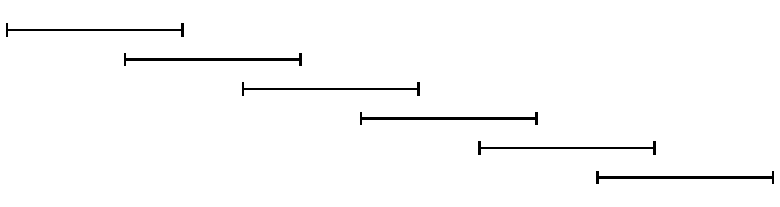
\includegraphics[width=0.7\textwidth]{fig90.pdf}
\end{center}

In diesem Beispiel gilt $p(j) = j-2$ für alle $j = 2,\ldots,n$. Für $j \geq 2$ erzeugt $\copt{(j)}$ also immer die rekursiven Aufrufe von $\copt{(j-1)}$ und von $\copt{(j-2)}$, d.h., die Gesamtzahl der rekursiven Aufrufe wächst wie die Fibonacci-Zahlen, welche \alert{exponentiell zunehmen.} (Man beachte, dass für die Fibonacci-Zahlen $f(0), f(1), f(2), \ldots$ gilt: $f(n+2) = f(n+1) + f(n) \geq 2f(n)$. Das heißt: $f(n+2)$ ist bereits mindestens doppelt so groß wie $f(n)$.)
\end{frame}

\begin{frame}
 \frametitle{Nur $n+1$ verschiedene Teilprobleme}
 Aufgrund der hohen Zahl der rekursiven Aufrufe können wir mit unserem Algorithmus alles andere als zufrieden sein. Trotzdem sind wir gar nicht so weit davon entfernt, unser Problem auf eine weitaus bessere Art zu lösen: \alert{Die entscheidende Beobachtung ist, dass unser rekursiver Algorithmus $\copt$ in Wirklichkeit nur $n+1$ verschiedene Teilprobleme löst:}
\[
\copt{(0)}, \ldots, \copt{(n)}.
\]

Als \alert{erste wichtige Komponente}, die bei einer Lösung mittels dynamischer Programmierung\label{page:13:1} vorhanden sein muss, hatten wir das \alert{Vorliegen einer Rekursionsgleichung} bezeichnet. Die \alert{zweite wichtige Komponente} haben wir soeben kennengelernt: Es muss eine Sammlung von \enquote{nicht allzu vielen}  Teilproblemen vorliegen, auf die sich die rekursiven Aufrufe beschränken.
\end{frame}

\begin{frame}
 \frametitle{Iterative Vorgehensweise}
 Das große Defizit unseres rekursiven Algorithmus lag in der extremen Häufigkeit, mit der immer wieder dieselben Teilprobleme aufgerufen werden. Wie kann man dies nun aber vermeiden? Es gibt zwei Möglichkeiten, die im Wesentlichen äquivalent sind: 
\begin{itemize}
\item Die eine nennt man \alert{Memoisation}; diese Möglichkeit soll hier nicht besprochen werden -- wir verweisen auf die Literatur (z.B. Kleinberg/Tardos oder Cormen et al.).
\item Die andere Möglichkeit ist, \alert{iterativ} vorzugehen.
\end{itemize}

Im Fall unseres Scheduling-Problems geht das wie folgt: Wir nutzen aus, dass die Teilprobleme bereits in einer sich anbietenden Reihenfolge vorliegen; deswegen benutzen wir ein Array $M[0 \ldots n]$ der Länge $n+1$, in dem die Werte $\opt{(0)}, \ldots, \opt{(n)}$ gespeichert werden. Beachtet man $\opt{(0)}=0$ sowie die Rekursionsformel \eqref{eq:13:1}, \alert{so ergibt sich der folgende iterative Algorithmus}.
\end{frame}

\begin{frame}
 \frametitle{Iterative-Compute-OPT}
 \begin{center}
\begin{tabular}{rl}
\multicolumn{2}{l}{$\mathbf{\icopt}$} \\
 (1)& $M[0] = 0$ \\
 (2)& \textbf{for} $j=1,\ldots,n$ \\
 (3)& \qquad $M[j] = \max\{ v_j + M[p(j)], M[j-1] \}$ \\
 (4)& \textbf{endfor}
\end{tabular}
\end{center} \medskip

Die \alert{Korrektheit} dieses Algorithmus ergibt sich aus (\ref{eq:13:1}) und $\opt{(0)}=0$. Die \alert{Laufzeit} von Iterative-Compute-Opt ist $O(n)$, da $n+1$ Einträge von $M[0 \ldots n]$ berechnet werden und die Berechnung jedes Eintrags in konstanter Zeit erfolgt. \\ \medskip

Wir greifen noch einmal das obige Beispiel aus Kleinberg/Tardos auf, um die Arbeitsweise von Iterative-Compute-OPT zu illustrieren:
\end{frame}

\begin{frame}
 \frametitle{Ein Beispiel}
 \begin{center}
  \includegraphics[width = 0.9\textwidth]{fig91.pdf}
 \end{center}
 
 \begin{center}
  \includegraphics[scale=0.8]{fig92.pdf}
 \end{center}

\end{frame}

\begin{frame}
 \frametitle{Bestimmung von $\O_n$}
 Möchte man nicht nur $\opt{(n)}$, sondern auch die dazugehörigen Intervalle der Menge $\O_n$ bestimmen, so ist dies auf der Basis von \eqref{eq:13:2} leicht möglich; die (einfachen) Details findet man im Buch von Kleinberg und Tardos. \\ \medskip

Unser Beispiel des gewichteten Intervall-Schedulings liefert eine \alert{grobe Richtlinie} für den Entwurf von Algorithmen mittels dynamischer Programmierung. Man benötigt vor allem eine \alert{Menge von Teilproblemen} des Ausgangsproblems, die gewissen Grundbedingungen genügen:  
\end{frame}

\begin{frame}
 \frametitle{Richtline}
 \begin{enumerate}[i)]
\item Es handelt sich um \alert{\enquote{nicht allzu viele} Teilprobleme.}
\item \alert{Die Lösung des Ausgangsproblems kann leicht aus den Lösungen der Teilprobleme berechnet werden.} (Einfachster Fall: Das Ausgangsproblem selbst befindet sich unter den Teilproblemen.)
\item \alert{Es gibt eine \enquote{natürliche Ordnung} unter den Teilproblemen sowie eine rekursive Beziehung}, die es erlaubt, die Lösung eines Teilproblems auf die Lösung von kleineren Teilproblemen zurückzuführen. (\enquote{Kleiner} bezieht sich dabei auf die erwähnte Ordnung.)
\end{enumerate}
\end{frame}

\begin{frame}
 \frametitle{Eine Vielzahl von interessanten Problemen}
 Natürlich ist dies nur eine informelle Richtlinie, die teilweise etwas vage bleiben muss. \alert{Die Schwierigkeit besteht meist darin, geeignete Teilprobleme zu einem gegebenen Problem aufzuspüren}. \\ \medskip

Eine Vielzahl von interessanten Problemen, die mit dynamischer Programmierung gelöst werden, findet man in den folgenden bekannten Lehrbüchern:
\begin{itemize}
\item Th. Cormen, Ch. Leiserson, R. Rivest, C. Stein: \textit{Introduction to Algorithms};
\item S. Dasgupta, Ch. Papadimitriou, U. Vazirani: \textit{Algorithms};
\item J. Kleinberg, É. Tardos: \textit{Algorithm Design}.
\end{itemize}
\end{frame}

\begin{frame}
\frametitle{Subset-Sum}
Wir haben das \structure{Rucksackproblem} (engl. \structure{Knapsack Problem}) bereits zuvor kennengelernt. Hier befassen wir uns zunächst mit einem \alert{Spezialfall des Rucksackproblems}, dass man das \structure{Subset-Sum-Problem} nennt. \\ \medskip
 
Gegeben seien $n$ \alert{Gegenstände}, die wir mit $1,\ldots,n$ bezeichnen wollen. Der Gegenstand $i$ habe das Gewicht $w_i \geq 0$, $w_i \in \Z$ ($i=1,\ldots,n$). Außerdem ist eine Schranke $W \geq 0$, $W \in \Z$ gegeben. Gesucht ist eine Teilmenge $S$ von $\{ 1,\ldots,n \}$, für die
\[
\sum\limits_{i \in S}{w_i} \leq W
\]
gilt und für die die links stehende Summe so groß wie möglich ist.
\end{frame}

\begin{frame}
 \frametitle{Subset-Sum-Problem vs. Rucksackproblem}
 Vergleichen wir das Subset-Sum-Problem mit dem Rucksackproblem, so stellen wir fest, dass es sich beim Subset-Sum-Problem um einen Sonderfall des Rucksackproblems (in binärer Variante) handelt: um den Spezialfall nämlich, dass $v_i=w_i$ gilt ($i=1,\ldots,n$). \\ \medskip
 
 Hier bezeichnet $v_i$ den \structure{Wert}  des Gegenstands $i$. 
 Mit \enquote{Rucksackproblem} meinen wir im Folgenden immer die Version 1 aus Vorlesung 3, bei der jeder Gegenstand nur einmal vorhanden ist (0,1-Problem). \\ \medskip
 
 Die deutsche Bezeichnung für Subset-Sum-Problem ist \structure{Teilsummenproblem}.
\end{frame}

\begin{frame}
 \frametitle{Entwurf eines Algorithmus}
 Zunächst: \alert{ein falscher Start}. \\ \medskip

Da wir das Problem mit dynamischer Programmierung behandeln wollen, müssen wir zunächst geeignete Teilprobleme finden. Wir orientieren uns am Problem des gewichteten Intervall-Schedulings und versuchen ähnlich vorzugehen, d.h., wir betrachten Teilprobleme der Form $\{ 1,\ldots,i \}$ und benutzen die Bezeichnung $\opt{(i)}$ analog zur Bedeutung in vorhergehenden Abschnitt. \\ \medskip

Mit $\O \subseteq \{ 1,\ldots,n \}$ wollen wir eine optimale Lösung des Subset-Sum-Problems bezeichnen. Ebenso wie beim gewichteten Intervall-Scheduling-Problem unterscheiden wir die beiden Fälle $n \notin \O$ und $n \in \O$. Der Fall $n \notin \O$ geht ebenso wie zuvor, d.h., wir können auch diesmal feststellen: 
\begin{itemize}
\item Falls $n \notin \O$, so gilt $\opt{(n)} = \opt{(n-1)}$.
\end{itemize}
\end{frame}

\begin{frame}
 \frametitle{Entwurf des Algorithmus}
 Nun zum Fall $n \in \O$. Beim gewichteten Intervall-Scheduling war auch dieser Fall einfach: Wir konnten alle Anfragen weglassen, die nicht kompatibel mit $n$ waren, und dann mit den restlichen Anfragen weiterarbeiten. \alert{Diesmal hat $n \in \O$ aber etwas anderes zur Folge}: \\ \medskip
 
 Die Aufnahme von $n$ in $\O$ impliziert, dass für die Gegenstände aus $\{ 1,\ldots,n-1 \}$ nur noch das Gewicht
\[
W-w_n
\]
zur Verfügung steht. Das bedeutet, dass es nicht ausreicht, Teilprobleme der Form $\{ 1,\ldots,i \}$ zu betrachten -- \alert{es müssen zusätzlich auch noch kleinere Schranken $w$ mit $0 \leq w \leq W$ Berücksichtigung finden.}
\end{frame}

\begin{frame}
 \frametitle{Modifikation des Ansatzes}
 \alert{Ganz so falsch war unser Start also doch nicht -- wir müssen unseren Ansatz nur modifizieren, indem wir weitere Teilprobleme hinzunehmen}. Dies wird im Folgenden durchgeführt. \\ \medskip

Wie wir gesehen haben, ist es also nötig, für jede Menge $\bigl\{ 1,\ldots,i \bigr\}$ von Gegenständen und für jede Gewichtsobergrenze $w$ mit $0 \leq w \leq W$ und $w \in \Z$ ein eigenes Teilproblem zu betrachten. Dementsprechend bezeichnen wir mit $\opt{(i,w)}$ das Gewicht einer optimalen Lösung des Subset-Sum-Problems für die Menge $\bigl\{ 1,\ldots,i \bigr\}$ und für das maximal zulässige Gewicht $w$. \\ \medskip

Man beachte, dass im Fall $w=0$ immer $\opt{(i,w)}=0$ gilt, da das maximal zulässige Gewicht gleich $0$ ist. Es gilt also immer $\opt{(i,0)}=0$. Darüber hinaus definiert man noch $\opt{(0,w)}=0$. (Dies entspricht dem einleuchtenden Umstand, dass das Gewicht einer optimalen Lösung gleich 0 ist, wenn keine Gegenstände vorhanden sind.)
\end{frame}

\begin{frame}
 \frametitle{Modifikation des Ansatzes}
 Für alle $i=0,\ldots,n$ und alle ganzen Zahlen $0 \leq w \leq W$ haben wir somit den Wert $\opt{(i,w)}$ definiert. Es sei daran erinnert, dass die Größe, die wir letzten Endes haben möchten, der Wert von $\opt{(n,W)}$ ist. Wie zuvor sei $\O \subseteq \bigl\{ 1,\ldots,n \bigr\}$ eine dazugehörige optimale Lösung. \\ \medskip
 
 Aufgrund unserer Überlegungen können wir feststellen:
\begin{itemize}
\item \alert{Falls $n \notin \O$, so gilt $\opt{(n,W)} = \opt{(n-1,W)}$.}
\item \alert{Falls $n \in \O$, so gilt $\opt{(n,W)} = w_n + \opt{(n-1,W-w_n)}$.}
\end{itemize} \medskip

Falls $W < w_n$ gilt, d.h., falls der $n$-te Gegenstand zu groß ist, so liegt klarerweise der Fall $n \notin \O$ vor und es gilt $\opt{(n,W)}=\opt{(n-1,W)}$. 
\end{frame}

\begin{frame}
 \frametitle{Die Rekursionsgleichung}
 Andernfalls ergibt sich, da einer der beiden Fälle $n \notin \O$ oder $n \in \O$ vorliegen muss:
\[
\alert{\opt{(n,W)} = \max\{ \opt{(n-1,W)}, w_n + \opt{(n-1, W-w_n)} \}}.
\]\medskip
 Entsprechendes gilt auch, wenn wir für $i \geq 1$ die Menge $\{ 1,\ldots,i \}$ anstelle von $\{ 1,\ldots,n \}$ sowie die Schranke $w$ anstelle von $W$ betrachten.
 \\ \medskip
 Somit erhalten wir das folgende Ergebnis (für $i \geq 1$):
\begin{equation}
\label{eq:13:3}
\opt{(i,w)} = \begin{cases}
\opt{(i-1,w)}, & \text{ für } w < w_i, \\
\max\{ \opt{(i-1,w)}, w_i + \opt{(i-1, w-w_i)} \}, & \text{ sonst.}
\end{cases}
\end{equation}

Damit haben wir die gewünschte \alert{Rekursionsgleichung} aufgestellt. 
\end{frame}

\begin{frame}
 \frametitle{Der Algorithmus}
 Anknüpfend an \eqref{eq:13:3} erhält man den folgenden Algorithmus zur Berechnung von $\opt{(n,W)}$:
\begin{center}
\begin{tabular}{rl}
\multicolumn{2}{l}{$\ssum{(n,W)}$} \\
 (1)& Array $M[0 \ldots n, 0 \ldots W]$ \\
 (2)& Initialisiere $M[0,w] = 0$ \textbf{für jedes} $w=0,\ldots,W$. \\
 (3)& \textbf{for} $i=1,\ldots,n$ \\
 (4)& \qquad \textbf{for} $w=0,\ldots,W$ \\ 
 (5)& \qquad\qquad Benutze die Rekursionsformel \eqref{eq:13:3} um $M[i,w]$ zu bestimmen. \\
 (6)& \qquad \textbf{endfor}\\
 (7)& \textbf{endfor} \\
 (8)& \textbf{return} $M[n,W]$.
\end{tabular}
\end{center}
Aufgrund von \eqref{eq:13:3} ergibt sich (durch vollständige Induktion), dass dieser Algorithmus korrekt ist, d.h., dass der gelieferte Wert von $M[n,W]$ gleich $\opt{(n,W)}$ ist.
\end{frame}

\begin{frame}
 \frametitle{Darstellung in einer Tabelle}
Ähnlich wie wir im Fall des gewichteten Intervall-Scheduling-Problems das Array $M$ in Form einer Tabelle dargestellt haben, deren Einträge schrittweise aus früheren Einträgen berechnet wurden, können wir uns $M$ auch diesmal als eine Tabelle vorstellen. \\ \medskip

\alert{Unterschied: Im vorliegenden Fall handelt es sich um eine 2-dimensionale Tabelle} (siehe nachfolgende Figur aus Kleinberg/Tardos), während wir es beim Intervall-Scheduling-Problem nur mit einer einzigen Zeile zu tun hatten.
\end{frame}

\begin{frame}
 \frametitle{Darstellung in einer Tabelle}
 \includegraphics[width=\textwidth]{fig93.pdf}
\end{frame}

\begin{frame}
 \frametitle{Ein Beispiel}
 Das folgende \textbf{Beispiel} aus Kleinberg/Tardos zeigt, wie die Tabelle zeilenweise von unten nach oben mit den Werten $\opt{(i,w)}$ aufgefüllt wird.
\begin{center}
 \includegraphics[scale=0.8]{fig94.pdf}
\end{center}
\end{frame}

\begin{frame}
 \frametitle{Zur Laufzeit}
 Es werden $(n+1)(W+1)$ Einträge berechnet und die Berechnung jedes Eintrags erfordert eine konstante Zahl von Operationen. Also beträgt die Laufzeit $O(nW)$. \alert{Damit ist der $\ssum$-Algorithmus nicht so effizient wie unser ebenfalls auf dynamischer Programmierung basierender Algorithmus zum gewichteten Intervall-Scheduling-Problem.} \\ \medskip
 
 Insbesondere handelt es sich \alert{\textbf{nicht} um einen polynomiellen Algorithmus.} \\ \medskip
 
 %\textbf{Man beachte:} Um die Schranke $W$ zu kodieren benötigt man lediglich $\left\lceil \log_2{(W+1)} \right\rceil$ Bits, während beim Aufstellen einer Zeile der 2-dimensionalen Tabelle $W+1$ Einträge zu berechnen sind. \\ \medskip
 
$\ssum{(n,W)}$ arbeitet jedoch effizient, wenn die Schranke $W$ im Vergleich zu $n$ nicht \enquote{übermäßig groß} ist\footnote{Man spricht von einem \structure{pseudo-polynomiellen Algorithmus}; Genaueres hierzu findet man beispielsweise im Buch von Kleinberg und Tardos.}.
\end{frame}

\begin{frame}
 \frametitle{Bestimmung der optimalen Menge $\O$ von Gegenständen}
 Der Algorithmus $\ssum{(n,W)}$ lässt sich leicht zu einem Algorithmus erweitern, der nicht nur den optimalen Wert $\opt{(n,W)}$ liefert, \alert{sondern auch eine dazugehörige optimale Menge $\O \subseteq \bigl\{ 1,\ldots,n \bigr\}$ von Gegenständen.}
 \begin{itemize}
 \item  Um $\O$ zu erhalten, führt man zunächst den Algorithmus $\ssum{(n,W)}$ wie beschrieben durch.
 \item Anschließend bestimmt man $\O$ mithilfe des Arrays $M[0 \ldots n, 0 \ldots W]$. Wir nehmen an, dass $M[0 \ldots n, 0 \ldots W]$ in Form einer Tabelle vorliegt, die -- wie zuvor beschrieben -- von unten nach oben aufgebaut wurde.
 \item Das von $\ssum{(n,W)}$ gelieferte Ergebnis ist dann der Eintrag $M[n,W]$, der in dieser Tabelle an der Stelle $[n,W]$ steht (\enquote{rechts oben}).
 \end{itemize}
\end{frame}

\begin{frame}
 \frametitle{Bestimmung der optimalen Menge $\O$ von Gegenständen}
 Ausgehend von der Stelle $[n,W]$ wandert man nun durch die Tabelle, bis man unten angekommen ist, wobei man nach der folgenden Regel verfährt:
 \begin{itemize}
 \item Steht man auf der Stelle $[i,w]$ für $i>0$ und gilt $M[i,w] = M[i-1,w]$, so nehme man $i$ nicht in $\O$ auf und gehe nach $[i-1,w]$;
 \item gilt dagegen $M[i,w] > M[i-1,w]$, so nehme man $i$ in $\O$ auf und gehe nach $[i-1,w-w_i]$.
 \end{itemize} \medskip

Nun sind wir auch nicht mehr weit davon entfernt, einen dynamischen-Programmierungs-Algorithmus für das \alert{Rucksackproblem} zu haben. \\ \medskip

\textbf{Kurz gesagt:} \alert{Beim Rucksackproblem läuft alles analog zum Subset-Sum-Problem; einziger Unterschied}: Es gilt nicht mehr unbedingt $v_i=w_i$. Dies wirkt sich nur insofern aus, dass man an einigen Stellen $v_i$ statt $w_i$ schreiben muss -- \alert{ansonsten bleibt alles beim Alten.}
\end{frame}

\begin{frame}
 \frametitle{Das Rucksackproblem}
 Das Rucksackproblem ist etwas komplexer als das Scheduling-Problem. Betrachte eine Situation in der jeder Gegenstand $i$ ein nichtnegatives Gewicht $w_i$ und einen individuellen Wert $v_i$ besitzt. Wir wollen eine Teilmenge $S$ \alert{maximalen Werts} $$\sum\limits_{i \in S}{v_i}$$ finden; unter der Einschränkung dass das Gewicht der Menge \alert{das Maximalgewicht $W$ nicht überschreitet}, also $$\sum\limits_{i \in S}{w_i} \leq W.$$
\end{frame}

\begin{frame}
 \frametitle{Das Rucksackproblem}
 Es ist nicht schwer, unseren dynamischen Programmierungsansatz auf dieses allgemeinere Problem zu erweitern. Wir verwenden eine analoge Menge von Teilproblemen, $\opt{(i, w)}$, \alert{um den Wert der optimalen Lösung durch eine Teilmenge der Gegenstände $\{1, \ldots, i \}$ und maximalem Wert $w$ zu bezeichnen.} \\ \medskip
 Wir betrachten eine optimale Lösung $\O$ und identifizieren zwei Fälle in Abhängigkeit davon, ob $n \in \O$ (oder $n \notin \O$):
\begin{itemize}
\item Falls $n \notin \O$, dann ist $\opt{(n,W)} = \opt{(n-1,W)}$.
\item Falls $n \in \O$, dann ist $\opt{(n,W)} = v_n + \opt{(n-1, W-w_n)}$.
\end{itemize}
\end{frame}

\begin{frame}
 \frametitle{Rekursionsformel für das Rucksackproblem}
 Diese Argumente für die Teilproblemem führen auf die Rekursionsformel
\begin{equation*}
\opt{(i,w)} = \begin{cases}
\opt{(i-1,w)}, & \text{ falls } w < w_i, \\
\max\{\opt{(i-1,w)}, v_i + \opt{(i-1,w-w_i)} \}, & \text{ sonst.}
\end{cases}
\end{equation*}

Auf diese Art und Weise können wir einen vollständig analogen dynamischen Programmierungsalgorithmus entwerfen und es gilt:

\begin{equation*}
\alert{\text{Das Rucksackproblem kann mit $O(nW)$ Aufwand gelöst werden.}}
\end{equation*}
\end{frame}

\end{document}
